\chapter{Bioinformática e análise de sequências}\label{ch:b3:bioinformatics}

Um biólogo que acaba de sequenciar um gene de um verme do mar profundo
cola seus \num{300} aminoácidos num formulário da web e, três segundos
depois, fica sabendo que a proteína é uma prima distante de uma cinase
humana, com \qty{31}{\%} de identidade ao longo de \num{280} resíduos
e uma probabilidade de $10^{-40}$ de a semelhança ser acaso. Por trás
desses três segundos estão um algoritmo de \omterm{thm:b3:bioinformatics:nw}{programação dinâmica} de
1970, uma teoria estatística dos \omterm{def:b3:bioinformatics:alignment}{alinhamentos} aleatórios, \omterm{def:b3:bioinformatics:matrices}{matrizes de
substituição} destiladas de milhares de famílias de proteínas e um
banco de dados de umas cem bilhões de posições. Este capítulo trata do
raciocínio dentro da caixa: como duas sequências são alinhadas de modo
que o \omterm{def:b3:bioinformatics:alignment}{alinhamento} seja comprovadamente o melhor, como o escore passa a
significar alguma coisa, como se distingue uma correspondência de uma
coincidência e como se acham padrões num genoma que ninguém examinou
antes. A matemática é elementar --- uma recorrência, um logaritmo, uma
distribuição de Poisson --- e vale a pena conhecê-la, porque toda
conclusão tirada de uma comparação de sequências repousa nela.

\section{Alinhar duas sequências}

\begin{definition}[Alinhamento e escore]\label{def:b3:bioinformatics:alignment}
\index{alinhamento de sequências}\index{penalidade de lacuna}\index{alinhamento global}\index{alinhamento local}
Um \emph{alinhamento} de duas sequências as escreve uma sobre a outra,
com \emph{lacunas} (--) inseridas de modo que as colunas emparelhem um
resíduo com um resíduo ou um resíduo com uma lacuna, e nenhuma coluna
emparelhe duas lacunas. Seu \emph{escore} é a soma, sobre as colunas,
de um escore de substituição $s(a,b)$ para cada par de resíduos e de
uma \emph{penalidade de lacuna} para cada lacuna: uma penalidade
linear $-d$ por posição de lacuna ou, mais realisticamente, uma
penalidade \emph{afim} $-d - (k-1)e$ para uma série de $k$ lacunas, com
o custo de abertura $d$ maior que o custo de extensão $e$, já que uma
inserção de vários resíduos é um único evento evolutivo. Um
alinhamento \emph{global} cobre as duas sequências de ponta a ponta; um
alinhamento \emph{local} encontra o par de subcadeias de maior escore e
ignora o resto, que é o que se quer quando um domínio compartilhado
está em duas proteínas de resto não aparentadas.
\end{definition}

\begin{theorem}[Needleman--Wunsch]\label{thm:b3:bioinformatics:nw}
\index{Needleman--Wunsch}\index{programação dinâmica}\index{Smith--Waterman}
Sejam $x = x_{1}\dots x_{m}$ e $y = y_{1}\dots y_{n}$, com penalidade
linear de lacuna $d$. Defina $F(i,j)$ como o melhor escore de um
\omterm{def:b3:bioinformatics:alignment}{alinhamento global} dos prefixos $x_{1}\dots x_{i}$ e $y_{1}\dots y_{j}$. Então $F(i,0) = -id$, $F(0,j) = -jd$ e, para $i,j \ge 1$,
\[
F(i,j) = \max\bigl\{\,F(i-1,j-1) + s(x_{i},y_{j}),\;
F(i-1,j) - d,\; F(i,j-1) - d\,\bigr\}.
\]
$F(m,n)$ é o escore global ótimo, um \omterm{def:b3:bioinformatics:alignment}{alinhamento} ótimo se recupera
retrotraçando a partir de $(m,n)$ as escolhas que produziram cada
máximo, e todo o cálculo leva $mn$ passos. A variante
\emph{Smith--Waterman} para \omterm{def:b3:bioinformatics:alignment}{alinhamento local} acrescenta $0$ como
quarta opção no máximo, fixa as bordas em $0$ e lê a resposta na maior
entrada da tabela.
\end{theorem}
\begin{proof}
Considere a última coluna de qualquer \omterm{def:b3:bioinformatics:alignment}{alinhamento} dos dois prefixos.
Ela é uma de três coisas: $x_{i}$ sobre $y_{j}$, $x_{i}$ sobre uma
lacuna, ou uma lacuna sobre $y_{j}$. Removê-la deixa um \omterm{def:b3:bioinformatics:alignment}{alinhamento} de
$(x_{1}\dots x_{i-1},
y_{1}\dots y_{j-1})$, de $(x_{1}\dots x_{i-1}, y_{1}\dots y_{j})$ ou de $(x_{1}\dots x_{i}, y_{1}\dots y_{j-1})$,
respectivamente, cujo escore é no máximo o $F$ desse par; e, ao
contrário, cada um desses \omterm{def:b3:bioinformatics:alignment}{alinhamentos} ótimos pode ser estendido pela
coluna final correspondente. Logo, o melhor escore que termina em cada
tipo de coluna é o $F$ do par mais curto mais o escore da coluna, e o
ótimo é o maior dos três. As bordas são forçadas (só lacunas são
possíveis contra um prefixo vazio). A indução sobre $i + j$ preenche a
tabela; o número de células é $(m+1)(n+1)$. Para o \omterm{def:b3:bioinformatics:alignment}{alinhamento local}, a
opção extra $0$ significa ``começar um novo \omterm{def:b3:bioinformatics:alignment}{alinhamento} aqui'', o que
faz de $F(i,j)$ o melhor escore de um \omterm{def:b3:bioinformatics:alignment}{alinhamento} que \emph{termina}
em $(i,j)$, e o melhor \omterm{def:b3:bioinformatics:alignment}{alinhamento local} termina em algum lugar.
\end{proof}

\begin{example}[Uma tabela quatro por três]\label{ex:b3:bioinformatics:nw-example}
Alinhe GAT com GCAT, pontuando $+1$ para correspondência, $-1$ para
discordância, $d = 1$. As bordas são $0, -1, -2, -3, -4$ ao longo do
topo e $0, -1,
-2, -3$ pela lateral. Preenchendo linha a linha:
$F(\text{G},\text{G}) = 1$,
$F(\text{G},\text{C}) = 0$, $F(\text{G},\text{A}) = -1$,
$F(\text{G},\text{T}) = -2$; $F(\text{A},\text{G}) = 0$,
$F(\text{A},\text{C}) = 0$, $F(\text{A},\text{A}) = 1$,
$F(\text{A},\text{T}) = 0$; $F(\text{T},\text{G}) = -1$,
$F(\text{T},\text{C}) = -1$, $F(\text{T},\text{A}) = 0$,
$F(\text{T},\text{T}) = 2$. O ótimo é $2$ e o retrotraçado
--- diagonal a partir de (T,T), diagonal a partir de (A,A), depois à
esquerda de (G,C) até (G,G), depois diagonal --- dá
\[
\begin{array}{c}
\texttt{G-AT}\\
\texttt{GCAT}
\end{array}
\]
três correspondências e uma lacuna: $3 - 1 = 2$.
\end{example}

\begin{omfigure}
\begin{tikzpicture}[every node/.style={font=\small}, >=stealth]
  \def\dx{1.0}\def\dy{0.8}
  % headers
  \foreach \j/\c in {1/G,2/C,3/A,4/T} \node[omDef, font=\small\bfseries] at (\j*\dx+0.5,0.4) {\c};
  \foreach \i/\c in {1/G,2/A,3/T} \node[omDef, font=\small\bfseries] at (-0.5,-\i*\dy-0.4) {\c};
  % grid
  \draw[gray!60] (0,0) grid[xstep=\dx, ystep=\dy] (5*\dx,-4*\dy);
  % values
  \foreach \i/\j/\v in {0/0/0,0/1/-1,0/2/-2,0/3/-3,0/4/-4,1/0/-1,2/0/-2,3/0/-3, 1/1/1,1/2/0,1/3/-1,1/4/-2, 2/1/0,2/2/0,2/3/1,2/4/0, 3/1/-1,3/2/-1,3/3/0,3/4/2}
    \node at (\j*\dx+0.5,-\i*\dy-0.4) {$\v$};
  % traceback path highlighted
  \foreach \i/\j in {0/0,1/1,1/2,2/3,3/4} \draw[omThm, very thick] (\j*\dx+0.05,-\i*\dy-0.05) rectangle (\j*\dx+\dx-0.05,-\i*\dy-\dy+0.05);
  \draw[->, omThm, very thick, shorten >=8pt, shorten <=8pt] (4.5,-2.8) -- (3.5,-2.0);
  \draw[->, omThm, very thick, shorten >=8pt, shorten <=8pt] (3.5,-2.0) -- (2.5,-1.2);
  \draw[->, omThm, very thick, shorten >=8pt, shorten <=8pt] (2.5,-1.2) -- (1.5,-1.2);
  \draw[->, omThm, very thick, shorten >=8pt, shorten <=8pt] (1.5,-1.2) -- (0.5,-0.4);
  \node[right, align=left] at (5.6,-1.6) {retrotraçado a partir de $F(3,4) = 2$:\\diagonal, diagonal,\\à esquerda (lacuna em GAT), diagonal\\[3pt] \texttt{G-AT}\\\texttt{GCAT}};
\end{tikzpicture}

{\small A tabela de Needleman--Wunsch para GAT contra GCAT
(correspondência $+1$, discordância $-1$, lacuna $-1$). Cada célula é o
melhor escore para os dois prefixos que ali terminam; o caminho
vermelho, retrotraçado a partir do canto, é o \omterm{def:b3:bioinformatics:alignment}{alinhamento} ótimo.}
\end{omfigure}

\begin{method}[Alinhar duas sequências]\label{met:b3:bioinformatics:align}
\index{retrotraçado}
(1) Escolha a pontuação: uma \omterm{def:b3:bioinformatics:matrices}{matriz de substituição} adequada à
divergência esperada (BLOSUM62 para proteínas de distância
desconhecida; correspondência/discordância para DNA) e penalidades
afins de lacuna (tipicamente abertura $-11$, extensão $-1$ com a
BLOSUM62). (2) Decida entre global e local: global para duas
sequências que se acreditam homólogas em todo o seu comprimento, local
nos demais casos. (3) Preencha a tabela pela recorrência, guardando
para cada célula um ponteiro para a escolha que deu seu máximo. (4)
Retrotrace a partir de $(m,n)$ (global) ou da célula máxima até um zero
(local), escrevendo o \omterm{def:b3:bioinformatics:alignment}{alinhamento} da direita para a esquerda. (5)
Julgue o resultado não por seu escore bruto, mas por sua significância
estatística (adiante), e olhe para ele: lacunas longas, trechos de
baixa complexidade e \omterm{def:b3:bioinformatics:alignment}{alinhamentos} confinados a uma repetição são
avisos.
\end{method}

\section{Pontuar: quanto vale uma correspondência}

\begin{definition}[Matrizes de substituição]\label{def:b3:bioinformatics:matrices}
\index{matriz de substituição}\index{BLOSUM}\index{PAM}\index{escore de log-chances}
Uma \emph{matriz de substituição} dá $s(a,b)$ para cada par de
aminoácidos como um \emph{escore de log-chances}:
\[
s(a,b) = \frac{1}{\lambda}\,\log\frac{q_{ab}}{p_{a}\,p_{b}},
\]
em que $q_{ab}$ é a frequência com que $a$ e $b$ são encontrados
alinhados em \omterm{def:b3:bioinformatics:alignment}{alinhamentos} confiáveis de proteínas aparentadas,
$p_{a} p_{b}$ é a frequência com que seriam emparelhados por acaso, e
$\lambda$ é uma escala escolhida para que as entradas sejam inteiros
convenientes. Um escore positivo significa que o par ocorre mais vezes
em homólogas do que por acaso; os escores de identidade são maiores
para os aminoácidos raros (triptofano $+11$, cisteína $+9$ na
BLOSUM62) e menores para os comuns (leucina $+4$, alanina $+4$), e as
substituições conservativas (isoleucina--valina $+3$) pontuam positivo
enquanto as radicais (triptofano--glicina $-2$) pontuam negativo. As
matrizes \emph{PAM} (Dayhoff, 1978) foram derivadas de proteínas
proximamente aparentadas e extrapoladas para distâncias maiores por
multiplicação de matrizes; as matrizes \emph{BLOSUM} (Henikoff e
Henikoff, 1992) foram contadas diretamente em blocos de sequências
alinhadas agrupadas a uma dada identidade --- a BLOSUM62 a partir de
blocos a \qty{62}{\%} --- e são o padrão porque foram medidas, e não
extrapoladas, na distância em que são usadas.
\end{definition}

\begin{proposition}[Por que log-chances]\label{prop:b3:bioinformatics:logodds}
\index{escore esperado}
Para que um esquema de pontuação possa ser usado em \omterm{def:b3:bioinformatics:alignment}{alinhamento local},
o \omterm{prop:b3:bioinformatics:logodds}{escore esperado} de uma coluna emparelhada ao acaso,
$\sum_{a,b} p_{a} p_{b}\, s(a,b)$, precisa ser negativo, e alguns
escores precisam ser positivos; do contrário os \omterm{def:b3:bioinformatics:alignment}{alinhamentos}
aleatórios cresceriam sem limite e o segmento de maior escore seria a
sequência inteira. Dado isso, qualquer esquema assim é equivalente a
um esquema de log-chances para \emph{algumas} frequências-alvo
$q_{ab}$ --- os \omterm{def:b3:bioinformatics:alignment}{alinhamentos} que ele achará ótimos são aqueles cujos
pares de resíduos se distribuem como $q_{ab}$. Escolher a matriz é,
portanto, escolher a divergência que se espera detectar: uma matriz
para parentes próximos (BLOSUM80, PAM30) tem positivos mais agudos e
negativos mais duros, e uma para parentes distantes (BLOSUM45, PAM250)
é mais achatada.
\end{proposition}
\admitted

\begin{example}[Identidade, similaridade e a zona crepuscular]\label{ex:b3:bioinformatics:twilight}
Duas sequências proteicas aleatórias alinhadas de forma ótima com
lacunas chegam a cerca de \qtyrange{15}{20}{\%} de identidade por
acaso. Acima de \qty{35}{\%} de identidade ao longo de cem resíduos,
duas proteínas são quase certamente homólogas; entre \qty{20}{\%} e
\qty{35}{\%} está a \emph{zona crepuscular}, em que a identidade
sozinha não decide e a estatística adiante precisa decidir. As
homólogas podem cair bem abaixo da zona: as subunidades da
hemoglobina e a mioglobina compartilham \qty{25}{\%} de identidade, a
lisozima e a $\alpha$-lactalbumina \qty{40}{\%}, e muitos pares de
proteínas de mesmo enovelamento compartilham menos de \qty{15}{\%},
detectáveis só pela comparação de perfis ou de estruturas.
\end{example}

\section{Buscar num banco de dados}

\begin{definition}[BLAST]\label{def:b3:bioinformatics:blast}
\index{BLAST}\index{semente}\index{par de segmentos de alto escore}
Alinhar uma consulta de \num{300} resíduos contra um banco de $10^{11}$
por \omterm{thm:b3:bioinformatics:nw}{programação dinâmica} completa custaria $3\times 10^{13}$
atualizações de célula por busca. O \emph{BLAST} (Altschul e
colaboradores, 1990) troca um pouco de sensibilidade por mil vezes mais
velocidade em três etapas: (1) lista as \emph{palavras} da consulta
(três resíduos para proteínas, onze bases para DNA) e suas vizinhas de
alto escore; (2) varre o banco em busca de correspondências exatas de
palavra --- as \emph{sementes}; (3) estende cada semente nos dois
sentidos sem lacunas até que o escore caia uma quantidade fixada abaixo
de seu melhor valor, guardando os \emph{pares de segmentos de alto
escore} (HSPs) e unindo depois os HSPs próximos por \omterm{thm:b3:bioinformatics:nw}{programação
dinâmica} com lacunas numa faixa estreita. Uma homóloga verdadeira quase
sempre contém ao menos uma palavra exata de três resíduos em comum; uma
semelhança de acaso raramente contém, e nunca é estendida.
\end{definition}

\begin{omfigure}
\begin{tikzpicture}[every node/.style={font=\scriptsize}, >=stealth]
  % query and database sequences as bars
  \draw[very thick, omDef] (0,2.0) -- (5,2.0); \node[left] at (-0.1,2.0) {consulta};
  \draw[very thick, gray] (0,0.6) -- (11,0.6); \node[left] at (-0.1,0.6) {banco de dados};
  % seeds
  \foreach \q/\d in {1.2/3.6, 2.8/5.2, 4.1/9.3} {
    \fill[omThm] (\q-0.15,1.9) rectangle (\q+0.15,2.1);
    \fill[omThm] (\d-0.15,0.5) rectangle (\d+0.15,0.7);
    \draw[omThm, thick] (\q,1.85) -- (\d,0.75);
  }
  \node[above] at (1.2,2.15) {palavra}; \node[above] at (2.8,2.15) {palavra}; \node[above] at (4.1,2.15) {palavra};
  % extension of the first two (same diagonal) -> HSP
  \draw[<->, very thick, omMeth!70!black] (2.6,0.3) -- (6.2,0.3); \node[below] at (4.4,0.25) {estender sem lacunas: um HSP};
  % third seed: extension fails
  \draw[omProp, thick, dashed] (8.8,0.3) -- (9.8,0.3); \node[below, omProp] at (9.3,0.25) {o escore cai: descartado};
  \node[right, align=left] at (5.5,2.0) {1. palavras da consulta\\2. acertos exatos no banco (sementes)\\3. estender, guardar os pares de alto escore};
\end{tikzpicture}

{\small A heurística do \omterm{def:b3:bioinformatics:blast}{BLAST}. Palavras exatas e curtas compartilhadas
pela consulta e pela entrada do banco (vermelho) são \omterm{def:b3:bioinformatics:blast}{sementes}; cada uma
é estendida ao longo de sua diagonal enquanto o escore continua
subindo, e só as extensões que se mantêm altas se tornam \omterm{def:b3:bioinformatics:blast}{pares de
segmentos de alto escore}.}
\end{omfigure}

\begin{theorem}[A estatística de um acerto ao acaso]\label{thm:b3:bioinformatics:evalue}
\index{valor E}\index{escore em bits}\index{Karlin--Altschul}
Para uma consulta de comprimento $m$ buscada contra um banco de
comprimento total $n$, com um esquema de pontuação de \omterm{prop:b3:bioinformatics:logodds}{escore esperado}
negativo, o número de \omterm{def:b3:bioinformatics:alignment}{alinhamentos} locais sem lacunas que pontuam ao
menos $S$ e surgem por acaso segue uma distribuição de Poisson de média
\[
E = K\,m\,n\,e^{-\lambda S},
\]
em que $\lambda$ e $K$ dependem apenas do esquema de pontuação e das
frequências dos resíduos ($\lambda$ é a escala da matriz de
log-chances). $E$ é o \emph{valor esperado} do escore $S$. Escrevendo o
escore em \emph{bits}, $S' = (\lambda S - \ln K)/\ln 2$, a fórmula se
torna $E = m n\, 2^{-S'}$, e a probabilidade de ao menos um \omterm{def:b3:bioinformatics:alignment}{alinhamento}
de acaso alcançar $S$ é $P = 1 - e^{-E}$, que é igual a $E$ quando $E$ é
pequeno.
\end{theorem}
\begin{proof}[Prova parcial]
A cauda exponencial é o teorema de Karlin--Altschul e é admitida: o
escore máximo de segmento de um passeio aleatório com deriva negativa
tem uma distribuição cuja cauda decai como $e^{-\lambda S}$, com
$\lambda$ a raiz positiva de
$\sum_{a,b} p_{a} p_{b} e^{\lambda s(a,b)} = 1$ --- que é exatamente a
equação que torna a matriz de log-chances consistente. Dada essa
cauda, o resto é contagem. Os segmentos de alto escore podem começar em
qualquer um dos $mn$ pares de posições, são raros e são quase
independentes; o número deles que excede $S$ é, portanto, Poisson com
média proporcional a $mn$ e à probabilidade da cauda,
$E = Kmn\,e^{-\lambda S}$. A probabilidade de nenhum é $e^{-E}$. A
substituição pelo \omterm{thm:b3:bioinformatics:evalue}{escore em bits} é álgebra: $e^{-\lambda S} K = 2^{-(\lambda S -
\ln K)/\ln 2}$. Para \omterm{def:b3:bioinformatics:alignment}{alinhamentos} com lacunas vale a
mesma forma, com $\lambda$ e $K$ estimados por simulação.
\end{proof}

\begin{example}[Ler um valor E]\label{ex:b3:bioinformatics:evalue}
Uma consulta de \num{250} resíduos contra um banco de $5\times 10^{10}$
resíduos tem $mn = 1.25\times 10^{13} \approx 2^{43.5}$. Um acerto com
\omterm{thm:b3:bioinformatics:evalue}{escore em bits} de $60$ tem $E = 2^{43.5 - 60} = 2^{-16.5} \approx 10^{-5}$: é, essencialmente com certeza, uma homóloga. Um acerto com
$S' = 40$ tem $E = 2^{3.5}
\approx 11$: esperam-se onze escores desses
por acaso, e o acerto não significa nada. O \emph{mesmo} \omterm{def:b3:bioinformatics:alignment}{alinhamento},
com o mesmo \omterm{thm:b3:bioinformatics:evalue}{escore em bits}, buscado contra um banco dez vezes maior,
tem um $E$ dez vezes maior --- a significância é propriedade da busca,
não do par. O limiar de uso comum é $E < 10^{-3}$ para uma homóloga
confiável; $E \approx 0.01$--$1$ merece uma segunda olhada com um
método de \omterm{def:b3:bioinformatics:msa}{perfil}.
\end{example}

\begin{omfigure}
\begin{tikzpicture}
\begin{axis}[
  width=0.7\linewidth, height=5.6cm,
  axis x line=bottom, axis y line=left,
  xmin=25, xmax=70, ymin=0.000000001, ymax=100000000, ymode=log,
  xlabel={escore em bits $S'$}, ylabel={$E$},
  xlabel style={font=\small, at={(axis description cs:0.5,-0.12)}, anchor=north},
  ylabel style={font=\small},
  tick label style={font=\small}, xtick={30,40,50,60,70},
  clip=false,
]
\addplot[very thick, omDef, domain=25:70, samples=2] {2^(43.5-x)};
\addplot[very thick, omThm, domain=25:70, samples=2] {2^(46.8-x)};
\addplot[dashed, gray, domain=25:70, samples=2] {0.001};
\node[font=\scriptsize, gray, anchor=south west] at (axis cs:25.5,0.0012) {$E = 10^{-3}$};
\node[font=\scriptsize, omDef, anchor=north west] at (axis cs:26,0.00002) {$mn = 1.25\times 10^{13}$};
\node[font=\scriptsize, omThm, anchor=south west] at (axis cs:45,30) {$mn$ dez vezes maior};
\end{axis}
\end{tikzpicture}

{\small $E = mn\,2^{-S'}$: cada bit a mais reduz à metade o número
esperado de acertos ao acaso, e um banco dez vezes maior custa $3.3$
bits de significância para o mesmo \omterm{def:b3:bioinformatics:alignment}{alinhamento}.}
\end{omfigure}

\section{Perfis, estados ocultos e motivos}

\begin{definition}[Alinhamento múltiplo e perfis]\label{def:b3:bioinformatics:msa}
\index{alinhamento múltiplo de sequências}\index{perfil}\index{modelo oculto de Markov de perfil}
Um \emph{\omterm{def:b3:bioinformatics:alignment}{alinhamento} múltiplo de sequências} organiza uma família de
sequências em colunas de resíduos homólogos. A \omterm{thm:b3:bioinformatics:nw}{programação dinâmica}
exata sobre $k$ sequências custa $n^{k}$ e é impossível além de três;
os programas práticos alinham \emph{progressivamente}, primeiro o par
mais próximo segundo uma árvore-guia, depois sequências e grupos ao
\omterm{def:b3:bioinformatics:alignment}{alinhamento} em crescimento, com rodadas de refinamento. Um \omterm{def:b3:bioinformatics:alignment}{alinhamento}
pronto é resumido como um \emph{perfil}: para cada coluna, a frequência
de cada resíduo e das lacunas. Um \emph{modelo oculto de Markov de
perfil} formaliza isso como uma cadeia de estados de correspondência,
um por coluna conservada, cada um emitindo resíduos com suas próprias
probabilidades, com estados de inserção e de deleção que admitem
resíduos a mais ou a menos em cada posição; o modelo de uma família
(uma entrada do Pfam) pontua uma nova sequência pela probabilidade do
melhor caminho pelos estados, e encontra homólogas bem abaixo da zona
crepuscular da comparação par a par, porque uma coluna que só tolera
resíduos hidrofóbicos diz isso, ao passo que uma sequência isolada não
pode dizer.
\end{definition}

\begin{omfigure}
\begin{tikzpicture}[every node/.style={font=\scriptsize}, >=stealth]
  % match states
  \foreach \i in {1,2,3,4} { \draw[thick, fill=omDef!25] (2.2*\i-0.5,0) rectangle (2.2*\i+0.5,0.7); \node at (2.2*\i,0.35) {M$_{\i}$}; }
  % insert states (diamonds) above
  \foreach \i in {1,2,3} { \draw[thick, fill=omProp!30] (2.2*\i+1.1,1.6) -- (2.2*\i+1.55,2.05) -- (2.2*\i+1.1,2.5) -- (2.2*\i+0.65,2.05) -- cycle; \node at (2.2*\i+1.1,2.05) {I$_{\i}$}; }
  % delete states (circles) below
  \foreach \i in {2,3} { \draw[thick, fill=gray!20] (2.2*\i,-1.3) circle (0.4); \node at (2.2*\i,-1.3) {D$_{\i}$}; }
  % transitions match->match
  \foreach \i in {1,2,3} \draw[->, thick] (2.2*\i+0.5,0.35) -- (2.2*\i+1.7,0.35);
  % match->insert->match
  \foreach \i in {1,2,3} { \draw[->, thick, omProp] (2.2*\i+0.3,0.7) -- (2.2*\i+0.9,1.65); \draw[->, thick, omProp] (2.2*\i+1.3,1.65) -- (2.2*\i+1.9,0.7); \draw[->, thick, omProp] (2.2*\i+1.1,2.5) arc[start angle=200, end angle=-20, radius=0.3]; }
  % match->delete->match
  \draw[->, thick, gray] (2.2+0.3,0) -- (4.4-0.3,-1.0); \draw[->, thick, gray] (4.4+0.3,-1.0) -- (6.6-0.3,0); \draw[->, thick, gray] (4.4+0.4,-1.3) -- (6.6-0.4,-1.3); \draw[->, thick, gray] (6.6+0.3,-1.0) -- (8.8-0.3,0);
  \node[below, align=center] at (2.2,-1.2) {emissões: uma distribuição de resíduos\\por estado de correspondência};
  \node[right, align=left] at (9.6,1.2) {uma sequência pontua por\\seu melhor caminho: correspondências,\\inserções (laranja) e\\deleções (cinza)};
\end{tikzpicture}

{\small Um \omterm{def:b3:bioinformatics:msa}{modelo oculto de Markov de perfil} de uma família de quatro
colunas. Cada estado de correspondência M emite um resíduo com as
frequências próprias da coluna; os estados de inserção I (com laços
sobre si) admitem resíduos extras, e os estados de deleção D saltam uma
coluna. Pontuar uma sequência é encontrar seu caminho mais provável.}
\end{omfigure}

\begin{definition}[Motivos e conteúdo de informação]\label{def:b3:bioinformatics:motif}
\index{motivo}\index{matriz de pesos por posição}\index{conteúdo de informação}\index{logo de sequência}
Um \emph{motivo} é um padrão curto --- um sítio de fator de
transcrição, um sinal de splicing, um sítio de fosforilação ---
representado por uma \emph{matriz de pesos por posição} com a
frequência $f_{i}(b)$ de cada base ou resíduo $b$ em cada posição $i$.
O \emph{conteúdo de informação} da posição $i$ é $R_{i} = 2 - H_{i}$
bits para o DNA, em que $H_{i} =
-\sum_{b} f_{i}(b)\log_{2} f_{i}(b)$ é sua entropia: $2$ bits para uma
base invariante, $0$ para uma posição em que as quatro são igualmente
prováveis. O total $R = \sum_{i} R_{i}$ é desenhado como um \emph{logo
de sequência}, cada posição uma pilha de letras cuja altura total é
$R_{i}$ e cujas letras têm tamanho proporcional à frequência.
\end{definition}

\begin{proposition}[Quanta informação um sítio precisa ter]\label{prop:b3:bioinformatics:bits}
\index{conteúdo de informação!e tamanho do genoma}
Um sítio que precisa ser encontrado $\gamma$ vezes num genoma de $G$
posições, e em nenhum outro lugar, precisa de cerca de
$R_{\text{necessário}} = \log_{2}(G/\gamma)$ bits de \omterm{def:b3:bioinformatics:motif}{conteúdo de
informação}: o \omterm{def:b3:bioinformatics:motif}{motivo} precisa reduzir as $G$ posições candidatas às
$\gamma$ verdadeiras, e cada bit reduz as candidatas à metade. Os
\omterm{def:b3:bioinformatics:motif}{motivos} observados de reguladores bacterianos bem estudados
correspondem a essa previsão --- os sítios de \emph{E.~coli} de um
repressor que se liga a algumas dezenas de lugares num genoma de
\qty{4.6}{Mb} carregam \numrange{16}{18} bits; os \omterm{def:b3:bioinformatics:motif}{motivos} de fatores de
transcrição eucariontes, com \numrange{8}{12} bits num genoma de
$3\times 10^{9}$, não conseguem especificar sozinhos seus alvos, e é
por isso que agem em combinações e na \omterm{def:b3:chromatin-epigenetics:nucleosome}{cromatina} aberta do
\cref{ch:b3:chromatin-epigenetics}.
\end{proposition}
\begin{proof}
Uma posição aleatória corresponde a um \omterm{def:b3:bioinformatics:motif}{motivo} de \omterm{def:b3:bioinformatics:motif}{conteúdo de informação}
$R$ com probabilidade de cerca de $2^{-R}$ (cada bit de especificidade
reduz a chance à metade), de modo que o número esperado de
correspondências ao acaso em $G$ posições é $G\,2^{-R}$. Para que os
sítios verdadeiros se destaquem, isso precisa ser da ordem de $\gamma$
ou menos: $G\,2^{-R} \le \gamma$, isto é, $R \ge \log_{2}(G/\gamma)$.
\end{proof}

\begin{example}[Correspondências esperadas ao acaso]\label{ex:b3:bioinformatics:motif-numbers}
Um sítio de restrição de seis bases fixas tem $R = 12$ bits e
corresponde a uma posição aleatória com probabilidade $4^{-6} = 2^{-12}$: cerca de \num{1100} vezes num genoma de \emph{E.~coli} de
\qty{4.6}{Mb} lido nas duas fitas (o sítio é palindrômico, e portanto
uma vez por posição) e $7\times 10^{5}$ vezes no genoma humano. Um
fator eucarionte cujo \omterm{def:b3:bioinformatics:motif}{motivo} carrega $10$ bits corresponde a
$3\times 10^{9}\times 2^{-10} \approx 3$ milhões de posições no genoma
humano, vários milhares de vezes mais do que os genes que ele regula.
Um \omterm{def:b3:bioinformatics:motif}{motivo} sozinho é um previsor fraco num genoma grande; o estado da
\omterm{def:b3:chromatin-epigenetics:nucleosome}{cromatina}, os \omterm{def:b3:bioinformatics:motif}{motivos} vizinhos e a conservação do sítio entre espécies
é que fazem uma previsão.
\end{example}

\begin{omfigure}
\begin{tikzpicture}[every node/.style={font=\scriptsize}]
  % sequence logo: TATA box-like 8 positions, stack heights = information content (1 bit = 1 cm)
  \draw[->] (0,0) -- (0,2.2); \node[left] at (-0.05,2.0) {2}; \node[left] at (-0.05,1.0) {1}; \node[left] at (-0.05,0) {0}; \node[rotate=90, above] at (-0.55,1.1) {bits};
  \draw (0,0) -- (8.6,0);
  \node[anchor=south, inner sep=0] at (0.5,0) {\resizebox{0.6cm}{1.9cm}{\textcolor{omThm}{\bfseries T}}};
  \node[anchor=south, inner sep=0] at (1.5,0) {\resizebox{0.6cm}{1.9cm}{\textcolor{omMeth!70!black}{\bfseries A}}};
  \node[anchor=south, inner sep=0] at (2.5,0) {\resizebox{0.6cm}{1.7cm}{\textcolor{omThm}{\bfseries T}}};
  \node[anchor=south, inner sep=0] at (3.5,0) {\resizebox{0.6cm}{1.9cm}{\textcolor{omMeth!70!black}{\bfseries A}}};
  \node[anchor=south, inner sep=0] at (4.5,0) {\resizebox{0.6cm}{1.0cm}{\textcolor{omMeth!70!black}{\bfseries A}}};
  \node[anchor=south, inner sep=0] at (4.5,1.0) {\resizebox{0.6cm}{0.4cm}{\textcolor{omThm}{\bfseries T}}};
  \node[anchor=south, inner sep=0] at (5.5,0) {\resizebox{0.6cm}{1.3cm}{\textcolor{omMeth!70!black}{\bfseries A}}};
  \node[anchor=south, inner sep=0] at (5.5,1.3) {\resizebox{0.6cm}{0.3cm}{\textcolor{omThm}{\bfseries T}}};
  \node[anchor=south, inner sep=0] at (6.5,0) {\resizebox{0.6cm}{0.5cm}{\textcolor{omProp}{\bfseries G}}};
  \node[anchor=south, inner sep=0] at (6.5,0.5) {\resizebox{0.6cm}{0.3cm}{\textcolor{omMeth!70!black}{\bfseries A}}};
  \node[anchor=south, inner sep=0] at (7.5,0) {\resizebox{0.6cm}{0.3cm}{\textcolor{omProp}{\bfseries G}}};
  \foreach \i in {1,...,8} \node[below] at (\i-0.5,-0.05) {\i};
  \node[below] at (4.3,-0.5) {posição no sítio};
\end{tikzpicture}

{\small Um \omterm{def:b3:bioinformatics:motif}{logo de sequência} de um \omterm{def:b3:bioinformatics:motif}{motivo} promotor do tipo caixa TATA.
A altura de cada pilha é o \omterm{def:b3:bioinformatics:motif}{conteúdo de informação} daquela posição,
$2 - H_{i}$ bits; as quatro primeiras posições são quase invariantes e
carregam a maior parte dos $12$ bits do \omterm{def:b3:bioinformatics:motif}{motivo}.}
\end{omfigure}

\section{Da sequência à função}

\begin{method}[Anotar uma proteína desconhecida]\label{met:b3:bioinformatics:annotate}
\index{domínio}\index{inferência de ortologia}
Dada uma nova sequência codificadora: (1) traduza-a na fase certa e
procure um peptídeo-sinal, segmentos transmembrana e regiões de baixa
complexidade; (2) busque nos bancos de proteínas com o \omterm{def:b3:bioinformatics:blast}{BLAST} e leia os
acertos com $E < 10^{-3}$, observando se o \omterm{def:b3:bioinformatics:alignment}{alinhamento} cobre a proteína
inteira (uma ortóloga verdadeira) ou um segmento (um domínio
compartilhado); (3) busque nos bancos de domínios com HMMs de \omterm{def:b3:bioinformatics:msa}{perfil},
que encontram famílias que o \omterm{def:b3:bioinformatics:blast}{BLAST} deixa passar e repartem a proteína
em domínios; (4) infira ortologia, e não mera similaridade, verificando
se o melhor acerto no outro genoma tem a consulta como \emph{seu}
melhor acerto (melhores acertos recíprocos) ou situando a proteína numa
árvore de genes (\cref{ch:b3:molecular-evolution}); (5) transfira a
função das ortólogas com cautela --- um resíduo catalítico conservado
argumenta a favor de uma química conservada, e um resíduo ausente
argumenta contra --- e preveja a estrutura; (6) trate toda previsão
como hipótese para a bancada.
\end{method}

\begin{proposition}[Estrutura a partir da sequência]\label{prop:b3:bioinformatics:structure}
\index{predição de estrutura}\index{modelagem por homologia}\index{coevolução}
O enovelamento de uma proteína é determinado por sua sequência
(\cref{ch:b3:structural-biology}), e calculá-lo a partir da sequência
foi durante cinquenta anos o problema central não resolvido da área.
Três abordagens tiveram êxito, uma após a outra. A \emph{\omterm{prop:b3:bioinformatics:structure}{modelagem por
homologia}} constrói a estrutura de uma proteína sobre a de uma homóloga
já resolvida, de modo confiável acima de \qty{30}{\%} de identidade. A
\emph{análise de coevolução} explora o fato de que dois resíduos em
contato no enovelamento tendem a mutar juntos ao longo de um
\omterm{def:b3:bioinformatics:alignment}{alinhamento} múltiplo profundo, de modo que pares de colunas
estatisticamente acopladas são contatos previstos, e contatos
bastantes definem um enovelamento. Os métodos de aprendizado profundo
treinados nas cem mil estruturas resolvidas e nesses \omterm{def:b3:bioinformatics:alignment}{alinhamentos} agora
preveem a maioria das estruturas de proteínas globulares com acurácia
quase experimental (as avaliações CASP de 2020), e há bancos com uma
estrutura prevista para praticamente toda sequência proteica conhecida.
O que eles preveem pior é aquilo que uma estrutura única não capta:
regiões desordenadas, conformações alternativas, o efeito de uma
mutação pontual e os complexos.
\end{proposition}

\begin{omfigure}
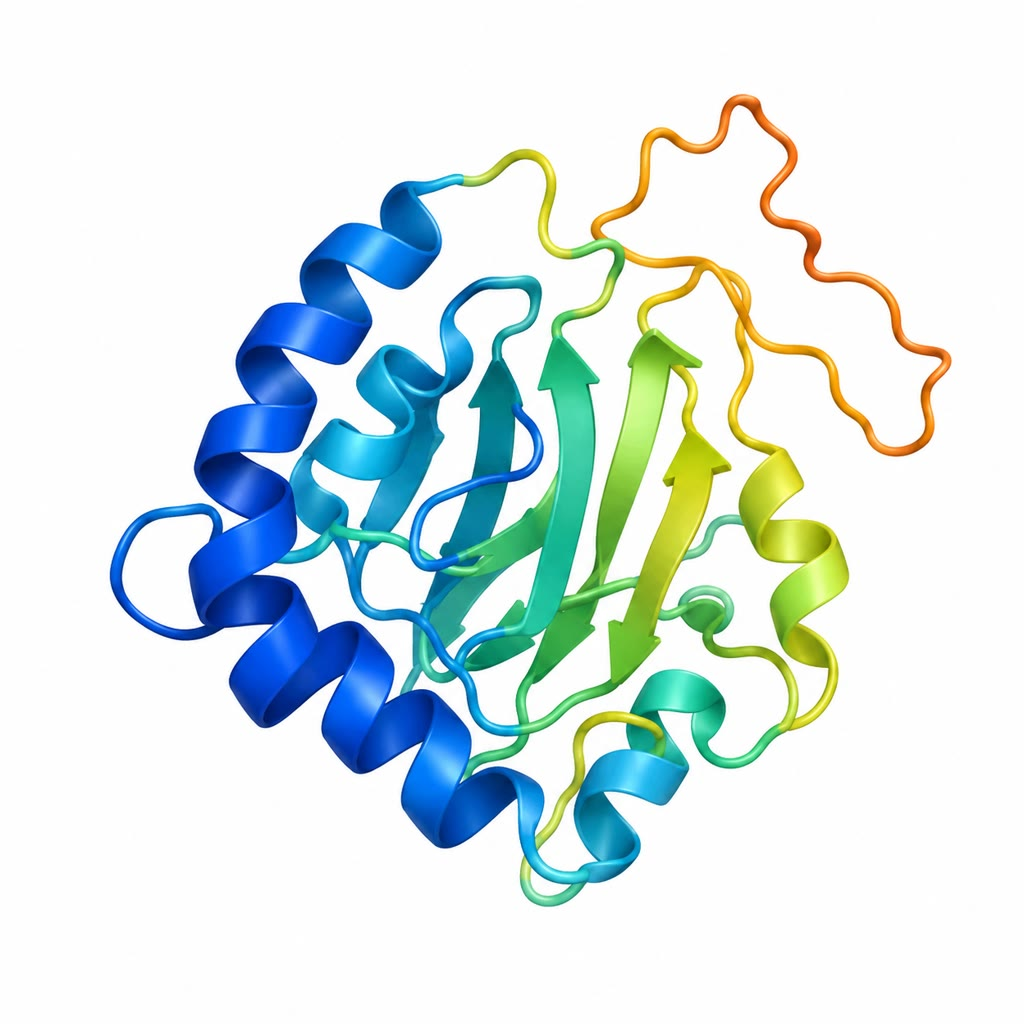
\includegraphics[width=0.36\linewidth]{images/book5/ai/b5-05-alphafold.jpg}\hspace{0.04\linewidth}
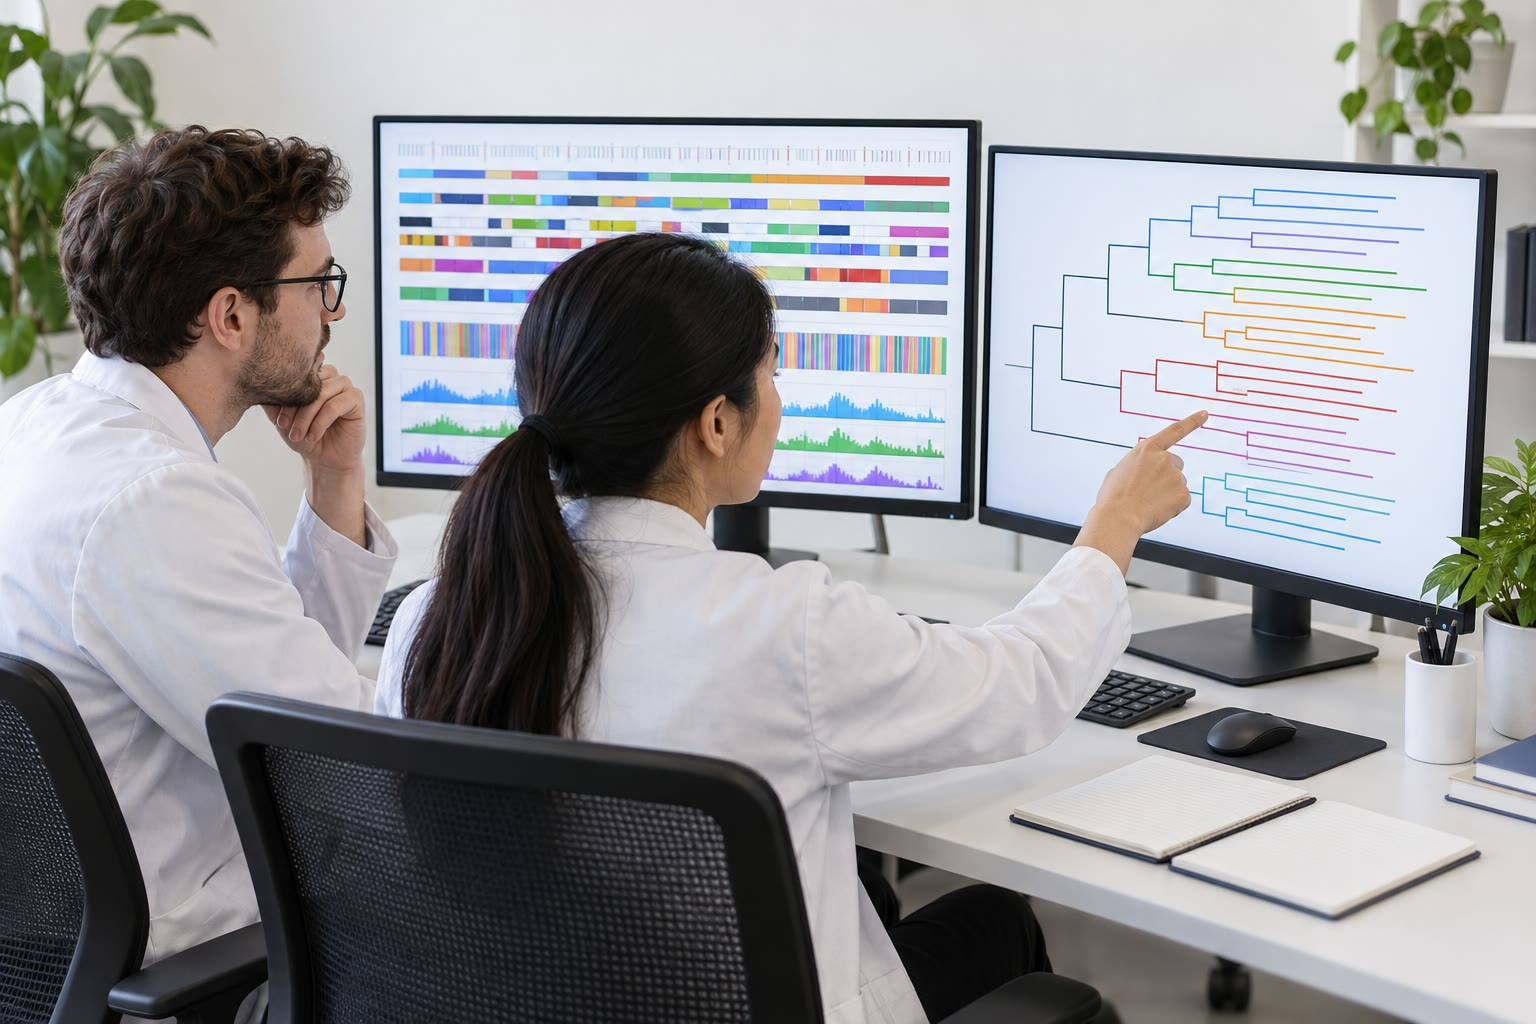
\includegraphics[width=0.54\linewidth]{images/book5/ai/b5-05-bioinformatics-lab.jpg}

{\small À esquerda: uma estrutura proteica prevista, colorida pela
confiança do modelo, de alta (azul) a baixa (laranja) numa alça
desordenada. À direita: um escritório de bioinformática --- navegadores
de genomas e árvores nas telas, e nenhuma bancada úmida à vista.}
\end{omfigure}

\begin{remark}[Os limites da inferência]\label{rem:b3:bioinformatics:limits}
A maioria das anotações funcionais nos bancos nunca foi testada; elas
foram transferidas de uma homóloga, que por sua vez fora anotada por
transferência. Os erros se propagam e se multiplicam, e uma \omterm{def:b3:genomics:assembly}{anotação}
errada numa proteína bem conectada pode infectar toda uma família. Os
remédios são os de cima: distinga ortologia de homologia, leia o
\omterm{def:b3:bioinformatics:alignment}{alinhamento}, procure os resíduos catalíticos e lembre que ``proteína
hipotética'' é um rótulo honesto que um terço dos genes da maioria dos
genomas ainda merece.
\end{remark}

\section{Exercícios}

\begin{exercise}[$\star$]\label{exo:b3:bioinformatics:1}
Defina \omterm{def:b3:bioinformatics:alignment}{alinhamento global} e local e dê uma situação biológica que
exija cada um.
\end{exercise}

\begin{exercise}[$\star$]\label{exo:b3:bioinformatics:2}
Preencha a tabela de Needleman--Wunsch para AGC contra AAC com
correspondência $+1$, discordância $-1$, lacuna $-1$, e dê o
\omterm{def:b3:bioinformatics:alignment}{alinhamento} ótimo e o escore.
\end{exercise}

\begin{exercise}[$\star$]\label{exo:b3:bioinformatics:3}
Na BLOSUM62, triptofano--triptofano pontua $+11$ e leucina--leucina
$+4$. Explique, a partir da fórmula de log-chances, por que a
identidade do resíduo mais raro vale mais.
\end{exercise}

\begin{exercise}[$\star$]\label{exo:b3:bioinformatics:4}
O que é um \omterm{thm:b3:bioinformatics:evalue}{valor E}? Uma busca devolve um acerto com $E = 3$. O que
esse número significa, e o acerto é uma homóloga?
\end{exercise}

\begin{exercise}[$\star\star$]\label{exo:b3:bioinformatics:5}
Uma consulta de \num{400} resíduos é buscada contra $2\times 10^{11}$
resíduos. Calcule o \omterm{thm:b3:bioinformatics:evalue}{valor E} de acertos com \omterm{thm:b3:bioinformatics:evalue}{escores em bits} $45$, $55$ e
$65$. Que \omterm{thm:b3:bioinformatics:evalue}{escore em bits} dá $E = 10^{-3}$? Como muda a resposta se a
consulta tiver \num{40} resíduos?
\end{exercise}

\begin{exercise}[$\star\star$]\label{exo:b3:bioinformatics:6}
Calcule o \omterm{def:b3:bioinformatics:motif}{conteúdo de informação} de um \omterm{def:b3:bioinformatics:motif}{motivo} cujas quatro posições têm
frequências de base (A, C, G, T) iguais a $(1,0,0,0)$,
$(0.5,0,0.5,0)$, $(0.25,0.25,0.25,0.25)$ e $(0.7,0.1,0.1,0.1)$.
Quantas correspondências ao acaso ele tem num genoma de \qty{4.6}{Mb}?
\end{exercise}

\begin{exercise}[$\star\star$]\label{exo:b3:bioinformatics:7}
Explique por que as penalidades afins de lacuna são mais realistas que
as lineares, e por que uma penalidade de abertura muito alta e uma
muito baixa dão, as duas, \omterm{def:b3:bioinformatics:alignment}{alinhamentos} ruins.
\end{exercise}

\begin{exercise}[$\star\star$]\label{exo:b3:bioinformatics:8}
Uma busca \omterm{def:b3:bioinformatics:blast}{BLAST} de uma proteína humana contra um banco de mosca dá um
melhor acerto com $E = 10^{-30}$ cobrindo os resíduos 50--180 da
consulta de \num{600} resíduos. A proteína da mosca é a ortóloga da
humana? Que teste adicional você faria?
\end{exercise}

\begin{exercise}[$\star\star$]\label{exo:b3:bioinformatics:9}
Por que os métodos de \omterm{def:b3:bioinformatics:msa}{perfil} detectam homólogas que o \omterm{def:b3:bioinformatics:alignment}{alinhamento} par a
par não detecta? Dê um exemplo de padrão de coluna que um \omterm{def:b3:bioinformatics:msa}{perfil} capta
e que uma sequência isolada não capta.
\end{exercise}

\begin{exercise}[$\star\star\star$]\label{exo:b3:bioinformatics:10}
Mostre que, sob um esquema de pontuação de \omterm{prop:b3:bioinformatics:logodds}{escore esperado} positivo, o
\omterm{def:b3:bioinformatics:alignment}{alinhamento local} de Smith--Waterman de duas sequências aleatórias
longas tem um escore que cresce linearmente com o comprimento delas, e
explique por que isso faz a teoria do \omterm{thm:b3:bioinformatics:evalue}{valor E} falhar. O que isso
implica para alinhar DNA com correspondência $+1$ e discordância $-1$
num conteúdo GC de \qty{60}{\%}?
\end{exercise}

\begin{exercise}[$\star\star\star$]\label{exo:b3:bioinformatics:11}
A tabela de Needleman--Wunsch precisa de $mn$ células de memória; para
dois cromossomos de \qty{100}{Mb} isso dá $10^{16}$. Descreva duas
ideias com que os alinhadores de genomas a evitam (\omterm{def:b3:bioinformatics:blast}{sementes} e
encadeamento; faixas) e o que cada uma abre mão.
\end{exercise}

\begin{exercise}[$\star\star\star$]\label{exo:b3:bioinformatics:12}
Um HMM de busca de genes em bactérias tem estados para as três posições
do códon e para o DNA não codificante. Explique como o modelo consegue
distinguir sequência codificadora de não codificante sem nenhuma
informação sobre códons de parada (considere o uso de códons), e por
que a mesma abordagem é muito mais difícil num genoma humano.
\end{exercise}

\section{Problema: uma sequência do mar profundo}

\begin{problem}[{Problema de fim de semana --- uma proteína desconhecida
alinhada à mão, buscada nos bancos com sua significância calculada, seu
motivo regulatório pesado em bits e seu gene conferido contra a
estatística das fases de leitura aberta aleatórias, terminando no valor
E do melhor acerto, nos bits de que um sítio precisa e no comprimento
que uma fase de leitura precisa ter para ser acreditada}]
\label{pb:b3:bioinformatics:1}
Dados: uma proteína de \num{300} resíduos de um anelídeo do mar
profundo. Banco de proteínas: $1.2\times 10^{11}$ resíduos. Genoma do
verme: \qty{1.6}{Gb}, \qty{38}{\%} GC. Pontuação dos \omterm{def:b3:bioinformatics:alignment}{alinhamentos} à
mão: correspondência $+1$, discordância $-1$, lacuna $-1$. \omterm{thm:b3:bioinformatics:evalue}{Escore em
bits} do melhor acerto do \omterm{def:b3:bioinformatics:blast}{BLAST}: $92$; do décimo acerto: $38$.
\medskip
\noindent\textbf{Parte I --- À mão.}
\begin{enumerate}
  \item Alinhe os peptídeos KQT e KAQT com a recorrência de
        Needleman--Wunsch: escreva a tabela e dê o \omterm{def:b3:bioinformatics:alignment}{alinhamento} ótimo e
        o escore.
  \item Repita com Smith--Waterman (local) para GATCAT contra ACAT:
        encontre o melhor \omterm{def:b3:bioinformatics:alignment}{alinhamento local} e seu escore.
  \item Quantas atualizações de célula custa um \omterm{def:b3:bioinformatics:alignment}{alinhamento global} da
        proteína de \num{300} resíduos contra uma proteína de
        \num{450} resíduos? E contra o banco inteiro?
  \item Se um computador faz $10^{9}$ atualizações por segundo, quanto
        tempo leva o \omterm{def:b3:bioinformatics:alignment}{alinhamento} da questão 3 contra o banco inteiro?
        Por que se usa o \omterm{def:b3:bioinformatics:blast}{BLAST} em vez dele?
  \item Um escore de identidade da BLOSUM62 é $+4$ para a alanina
        ($p_{A} =
        0.074$) e $+11$ para o triptofano ($p_{W} = 0.013$).
        Com $\lambda = 0.347$ (unidades de meio bit), calcule a
        frequência-alvo $q_{AA}$ e $q_{WW}$, e a razão $q/p^{2}$ de
        cada uma. Interprete.
  \item Duas proteínas compartilham \qty{24}{\%} de identidade ao longo
        de $250$ resíduos. Diga por que a identidade sozinha não
        resolve a homologia aqui e o que resolveria.
\end{enumerate}

\medskip
\noindent\textbf{Parte II --- A busca.}
\begin{enumerate}[resume]
  \item Calcule $mn$ para a consulta contra o banco, e $\log_{2}(mn)$.
  \item Calcule o \omterm{thm:b3:bioinformatics:evalue}{valor E} do melhor acerto ($S' = 92$) e do décimo
        acerto ($S' = 38$).
  \item Que \omterm{thm:b3:bioinformatics:evalue}{escore em bits} corresponde a $E = 10^{-3}$ nesta busca? E a
        $E = 1$?
  \item O mesmo melhor acerto é encontrado quando o banco cresceu para
        $1.2\times 10^{12}$ resíduos. Seu \omterm{thm:b3:bioinformatics:evalue}{valor E}?
  \item O décimo acerto alinha os resíduos 200--260 da consulta com
        \qty{40}{\%} de identidade ao longo de $60$ resíduos. Usando o
        \omterm{thm:b3:bioinformatics:evalue}{valor E}, diga se ele é evidência de homologia e o que uma busca
        por \omterm{def:b3:bioinformatics:msa}{perfil} poderia acrescentar.
  \item O melhor acerto é uma cinase humana, alinhada ao longo dos
        resíduos 10--290. Seu melhor acerto no proteoma do verme é a
        consulta. O que esse teste recíproco estabelece, e o que não
        estabelece?
\end{enumerate}

\medskip
\noindent\textbf{Parte III --- Um \omterm{def:b3:bioinformatics:motif}{motivo}.}
\begin{enumerate}[resume]
  \item A montante do gene há um candidato a sítio de fator de
        transcrição de oito posições com \omterm{def:b3:bioinformatics:motif}{conteúdos de informação}
        $2, 2, 1.6, 2, 0.8, 1.2, 0.4, 0.3$ bits. Qual é o $R$ total?
  \item Quantas correspondências ao acaso o \omterm{def:b3:bioinformatics:motif}{motivo} tem no genoma de
        \qty{1.6}{Gb} (as duas fitas, $3.2\times 10^{9}$ posições)?
  \item O fator regula cerca de $200$ genes. De quantos bits um \omterm{def:b3:bioinformatics:motif}{motivo}
        precisaria para especificar sozinho $200$ sítios neste genoma?
  \item Quanto dessa falta um segundo \omterm{def:b3:bioinformatics:motif}{motivo} adjacente de $8$ bits
        poderia suprir, se os dois precisarem ocorrer juntos dentro de
        um espaçamento fixo?
  \item Uma posição com frequências $(0.5, 0.5, 0, 0)$ para (A, C, G,
        T): calcule sua entropia e seu \omterm{def:b3:bioinformatics:motif}{conteúdo de informação}.
  \item Explique, com o argumento de informação, por que os fatores de
        transcrição bacterianos costumam ter sítios mais longos e mais
        conservados que os eucariontes.
\end{enumerate}

\medskip
\noindent\textbf{Parte IV --- O próprio gene.}
\begin{enumerate}[resume]
  \item Em DNA aleatório de composição de bases uniforme, qual é a
        probabilidade de um códon ser de parada? Qual é o número
        esperado de códons antes que apareça um de parada (uma
        distribuição geométrica)?
  \item O genoma do verme tem \qty{38}{\%} GC. Recalcule a
        probabilidade de um códon aleatório ser de parada (TAA, TAG,
        TGA) com as frequências de base reais, e o comprimento
        esperado da fase de leitura. Em que direção um conteúdo GC
        baixo empurra a busca de genes?
  \item Qual é a probabilidade de uma fase de leitura aberta aleatória
        ter ao menos $100$ códons? E ao menos $300$?
  \item No genoma de \qty{1.6}{Gb}, seis fases em duas fitas dão cerca
        de $3.2\times 10^{9}$ inícios de códon. Quantas fases de
        leitura aberta aleatórias de ao menos $100$ códons se esperam?
        E de ao menos $300$?
  \item Explique por que ``fase de leitura aberta com mais de $100$
        códons'' é um localizador de genes utilizável numa bactéria,
        mas não neste genoma, e o que um localizador de genes
        eucarionte usa em vez disso.
  \item O gene do verme tem seis éxons de \qty{150}{bp} em média.
        Explique como as leituras de sequenciamento de RNA resolvem a
        estrutura de éxons que a sequência genômica sozinha deixa
        ambígua.
  \item Resuma: o \omterm{thm:b3:bioinformatics:evalue}{valor E} do melhor acerto (questão~8), os bits
        necessários para especificar $200$ sítios (questão~15) e o
        número esperado de fases de leitura aleatórias de $300$ códons
        no genoma (questão~22).
\end{enumerate}
\end{problem}
